\ylDisplay{Õhuhoki} % Ülesande nimi
{Mihkel Heidelberg} % Autor
{lõppvoor} % Voor
{2010} % Aasta
{G 6} % Ülesande nr.
{5} % Raskustase
{
% Teema: Gaasid
\ifStatement
Heast soojusjuhist plaadile asetatakse kuivast jääst (st tahkest
süsihappegaasist) kerge seib raadiusega $r=\SI{1}{cm}$; seibi surutakse
pealt jõuga $F=\SI{10}{N}$. Millise minimaalse aluse
temperatuuri juures hõljub seib sublimeeruva süsihappegaasi tekitatud
gaasipadjal? Aluse temperatuur lugege ühtlaseks ja samaks temaga
vahetus kontaktis oleva ainekihiga. Õhurõhk $p_{0}=\SI{100}{kPa}$
ja kuiva jää aururõhu sõltuvus temperatuurist on kujutatud graafikul.

\begin{center}
	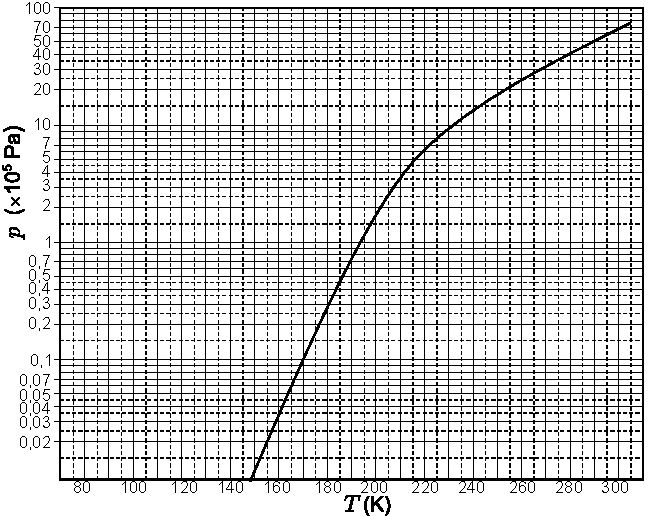
\includegraphics{2010-v3g-06-Aururohk}
\end{center}
\fi


\ifHint
Seibi alumise külje läheduses surub süsihappegaas teatud rõhuga seibi ülesse. Vastav jõud on ülemiselt küljelt tasakaalustatud nii õhurõhu, kui ka surumisjõu poolt.
\fi


\ifSolution
Olukorras, kus aluse temperatuur on minimaalne, on rõhk seibi alumise külje vahetus läheduses võrdne
süsihappegaasi aururõhuga. Seibi surutakse alla jõuga $F$ ja kuna seibi
pindala on $\pi r^2$, peab surumist tasakaalustav rõhk olema $p={F\over \pi r^2}$.
Vaadeldes rõhkude tasakaalu seibi ülemise ja alumise pinna läheduses, saame et kuiva jää aururõhk on
\[
p\idx{kuiv} = p + p_0= p_0+{F\over \pi r^2} = \SI{131.8}{kPa}.
\]
Sellele vastab graafiku põhjal temperatuur $\sim \SI{195}{K}$.
\fi
}